\documentclass{article}
\usepackage[utf8]{inputenc}

\usepackage{amssymb}
\usepackage{graphicx}
\title{Rapport TP2}

\author{Yu Deng, 20151659\\Rosine Rolande Simo Tegninko, }

\date{October 2022}

\begin{document}

\maketitle

\section{GQM}\\


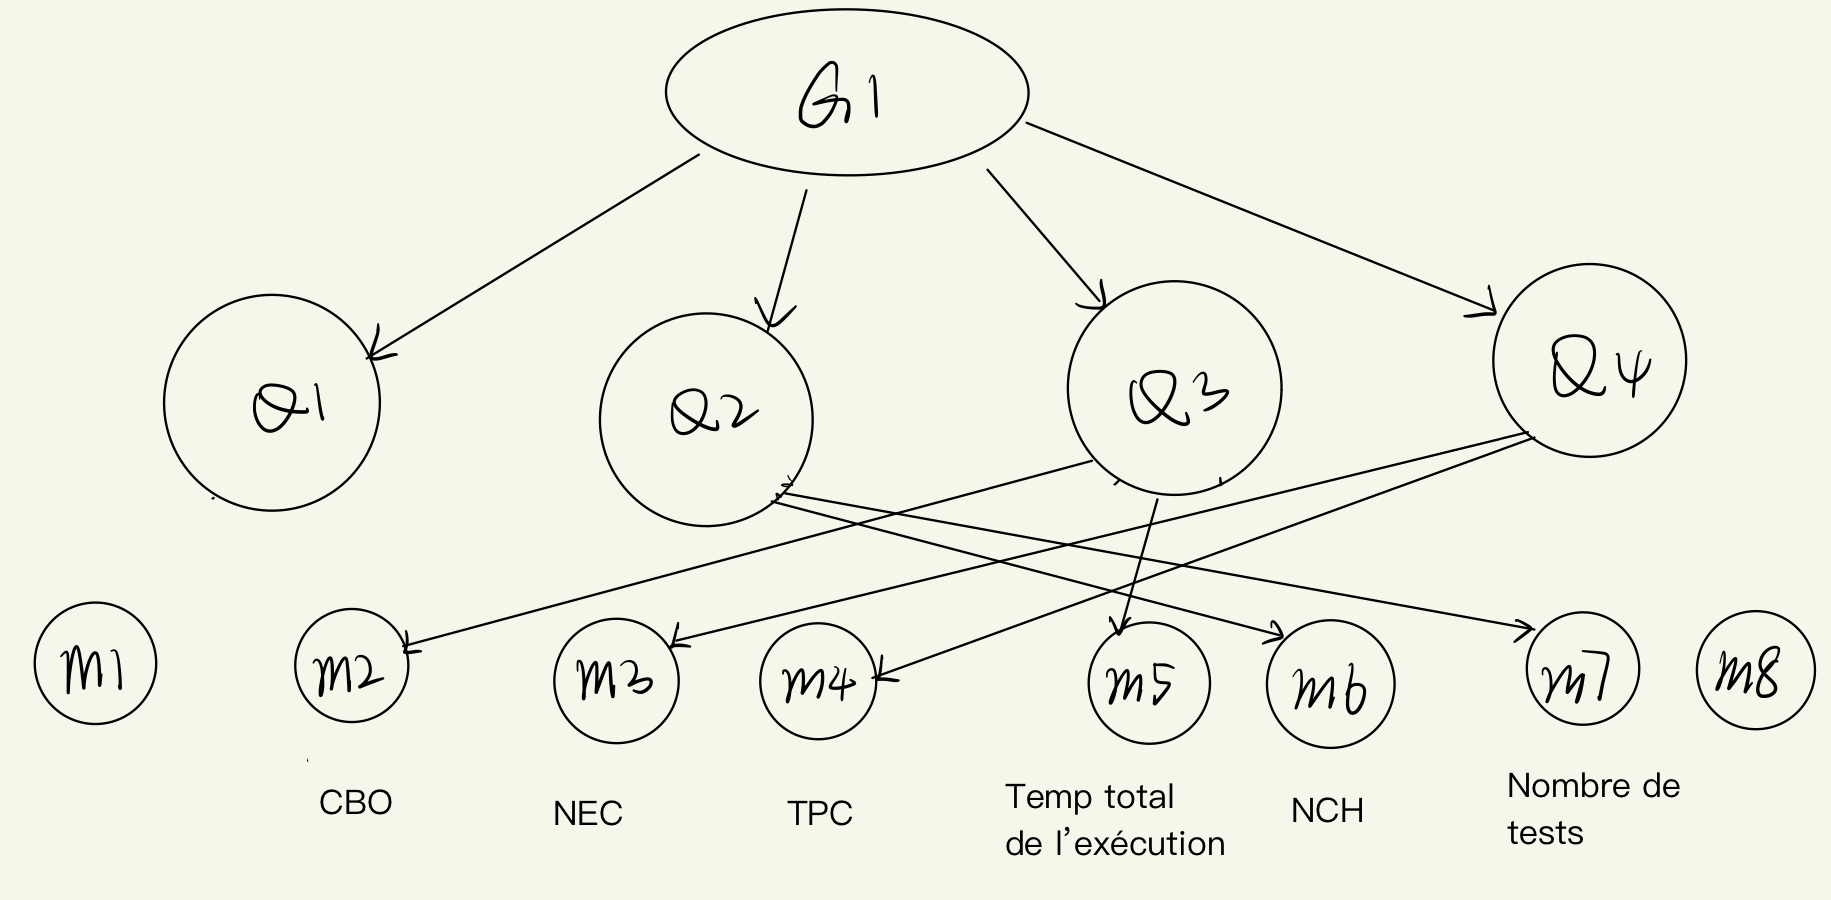
\includegraphics[scale=0.2]{image.jpg} \\

\item(Q1)\\

Le niveau de documentation des classes est-il approprié par rapport à leur complexité ?\\


\item(Q2)\\

La conception est-elle bien modulaire ?\\

Pour le Q2, nous avons choisi deux métriques, NCH et Nombre de tests.\\

1.	NCH fait référence au nombre de commits dans l'historique de la classe. Ensuite, nous pouvons juger s'il est adapté à sa complexité en regardant le nombre de commits. Voici pourquoi : s'il y a trop de commits, alors on sait aussi que la personne qui a écrit ce code le met constamment à jour afin de pouvoir l'adapter à la complexité.\\

2.Plusieurs tests sont sûrs de trouver de nombreux problèmes. Et pour chaque test, nous devons "augmenter" la complexité de "l'entrée" pour détecter si le niveau de document de la classe est approprié à sa complexité.\\

\item(Q3)\\

Le code est-il mature ?\\

###Pour Q3, nous avons sélectionné deux métriques, CBO et Temps total de l’exécution.\\

1. CBO fait référence à "Coupling Between Objects", nous savons que plus une classe est couplée à d'autres classes, plus une modification de cette classe peut influencer de classes. Ensuite, CBO a joué un grand rôle en testant si le code est mature, If ce code peut avoir un CBO inférieur, la charge de travail des tests sera également réduite, ce qui montre déguisé que ce code a été modifié plusieurs fois et est relativement mature. Ensuite, cela n'affectera pas plusieurs aspects en raison de tâches de test fastidieuses.\\

2. Pour Temps total de l’exécution, lorsque nous testons, le résultat est très lent. Tout le monde veut obtenir une réponse le plus rapidement possible, ensuite si le temps d'exécution est lent, le code est moins mature et moins adapté aux besoins des gens.\\


\item(Q4)\\

 Le code peut-il être testé bien automatiquement ?\\
 
 Pour le Q4, nous avons choisi deux métriques, TPC et NEC.\\

1. Pour TPC, nous testons en fonction de la classe, donc au lieu de tester directement l'intégralité du code, nous pouvons juger si chaque partie peut être exécutée correctement grâce à des tests automatiques. S'il y a un bogue dans l'un d'entre eux, alors lorsque le code global est automatiquement testé, certains bogues seront trouvés.\\

2. Pour NEC, il est évident que si un code a beaucoup d'erreurs après son exécution, alors le code doit avoir une erreur dans un certain lien. Lors du test automatique, il a dû rencontrer des problèmes, ensuite, ce code ne fonctionne pas bien dans les tests automatiques.\\



\end{document}
